\documentclass[12pt,letterpaper]{article}
\usepackage[utf8]{inputenc}
\usepackage[spanish]{babel}
\usepackage{graphicx}
\usepackage[left=2cm,right=2cm,top=2cm,bottom=2cm]{geometry}
\usepackage{graphicx} % figuras
% \usepackage{subfigure} % subfiguras
\usepackage{float} % para usar [H]
\usepackage{amsmath}
%\usepackage{txfonts}
\usepackage{stackrel} 
\usepackage{multirow}
\usepackage{enumerate} % enumerados
\renewcommand{\labelitemi}{$-$}
\renewcommand{\labelitemii}{$\cdot$}
% \author{}
% \title{Caratula}
\begin{document}

% Fancy Header and Footer
% \usepackage{fancyhdr}
% \pagestyle{fancy}
% \cfoot{}
% \rfoot{\thepage}
%

% \usepackage[hidelinks]{hyperref} % CREA HYPERVINCULOS EN INDICE

% \author{}
\title{Caratula}

\begin{titlepage}
\begin{center}
\large{UNIVERSIDAD PRIVADA-DE-TACNA}\\
\vspace*{-0.025in}
\begin{figure}[htb]
\begin{center}

\includegraphics[width=8cm]{./Imagenes/logo}
\end{center}
\end{figure}
\vspace*{0.15in}
INGENIERIA DE SISTEMAS  \\

\vspace*{0.5in}
\begin{large}
TITULO:\\
\end{large}

\vspace*{0.1in}
\begin{Large}
\textbf{Practica de laboratorio Nr 02: Modelado Datos en Power Bi} \\
\end{Large}

\vspace*{0.3in}
\begin{Large}
\textbf{CURSO:} \\
\end{Large}

\vspace*{0.1in}
\begin{large}
Inteligencia de Negocios\\
\end{large}

\vspace*{0.3in}
\begin{Large}
\textbf{DOCENTE(ING):} \\
\end{Large}

\vspace*{0.1in}
\begin{large}
 Patrick Cuadros Quiroga\\
\end{large}

\vspace*{0.2in}
\vspace*{0.1in}
\begin{large}
Integrante: \\
\begin{flushleft}
Andre Sebastian Reinoso Aranda          	\hfill	(2016055275) \\

\end{flushleft}
\end{large}
\end{center}

\end{titlepage}


\tableofcontents % INDICE
\thispagestyle{empty} % INDICE SIN NUMERO
\newpage
\setcounter{page}{1} % REINICIAR CONTADOR DE PAGINAS DESPUES DEL INDICE

\section{Proceso} 

\begin{itemize}
	\item Relacion entre tablas del excel
	\begin{center}
	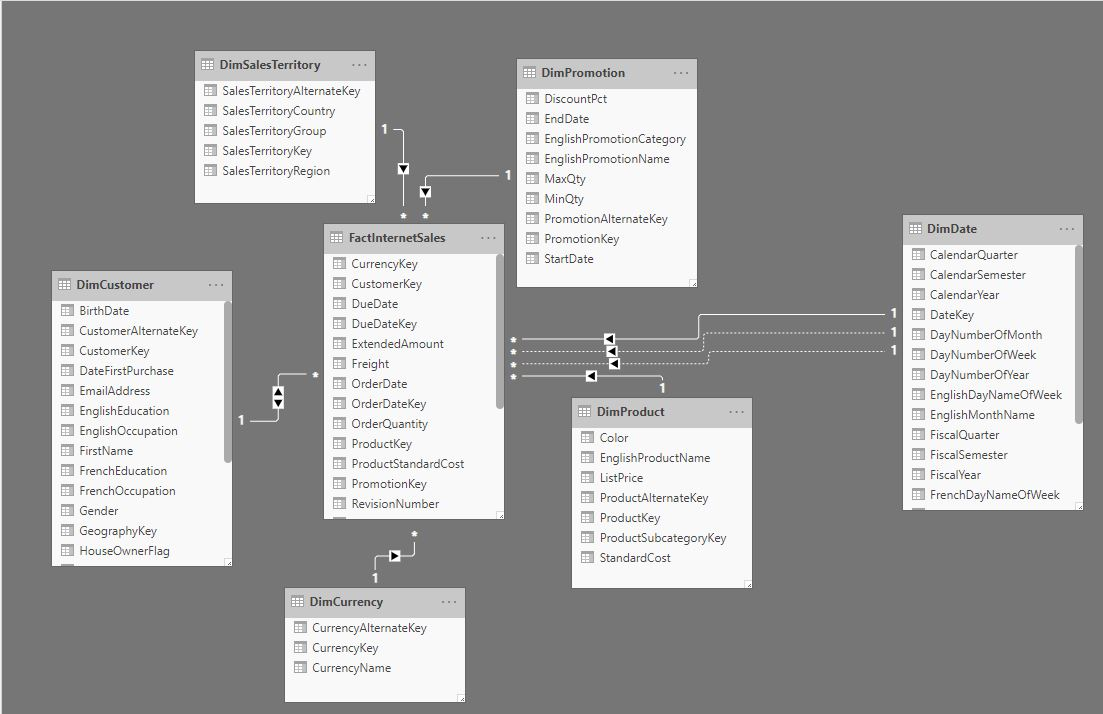
\includegraphics[width=10cm]{./Imagenes/1} 
	\end{center}
\end{itemize} 

\begin{itemize}
	\item Relacion de las tablas despues de agregar el nuevo excel
	\begin{center}
	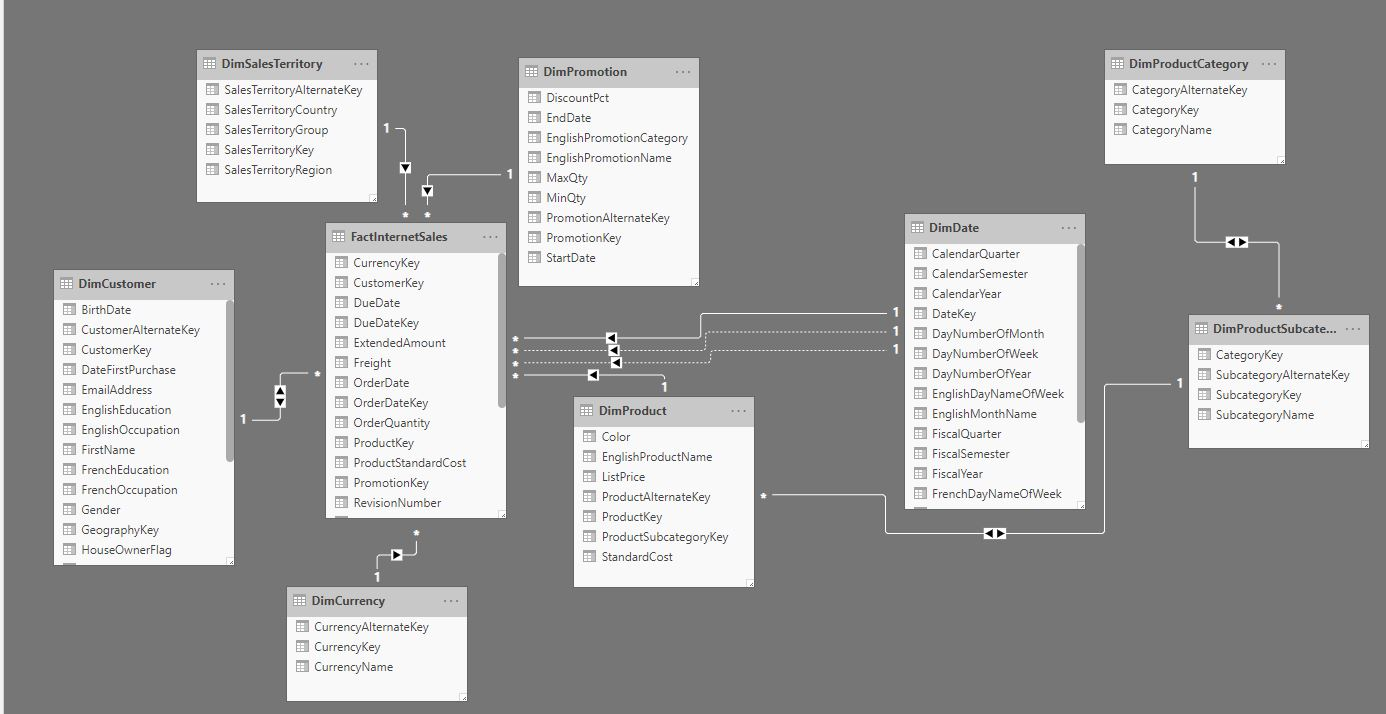
\includegraphics[width=10cm]{./Imagenes/2} 
	\end{center}
\end{itemize} 

\begin{itemize}
	\item Calculo de columna en DimCustomer
	\begin{center}
	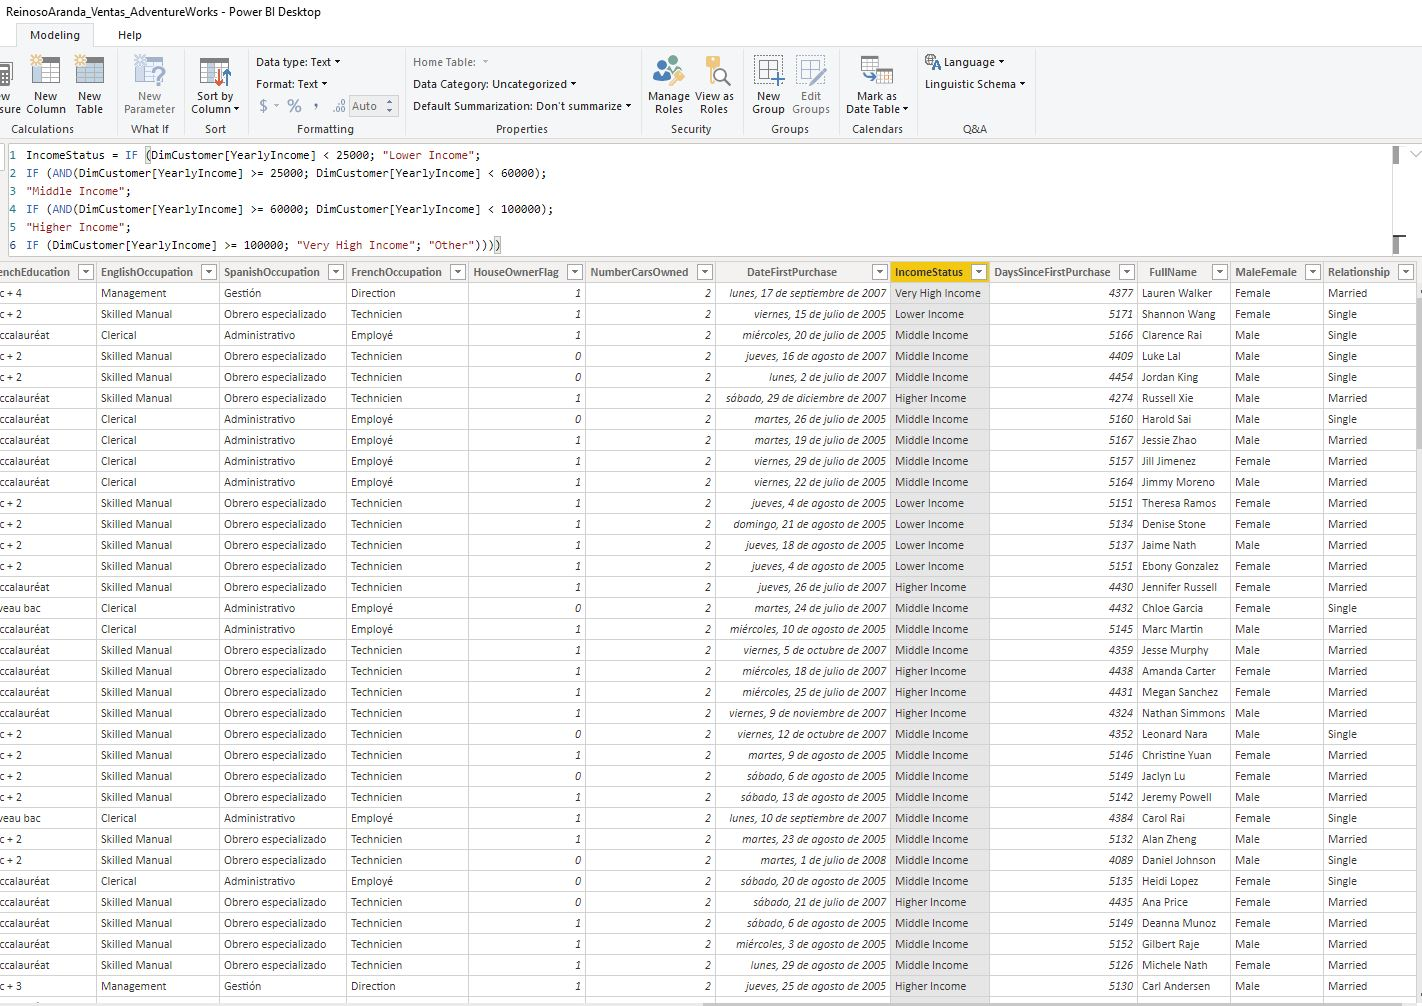
\includegraphics[width=10cm]{./Imagenes/3} 
	\end{center}
\end{itemize} 

\begin{itemize}
	\item Relaciones de las tablas
	\begin{center}
	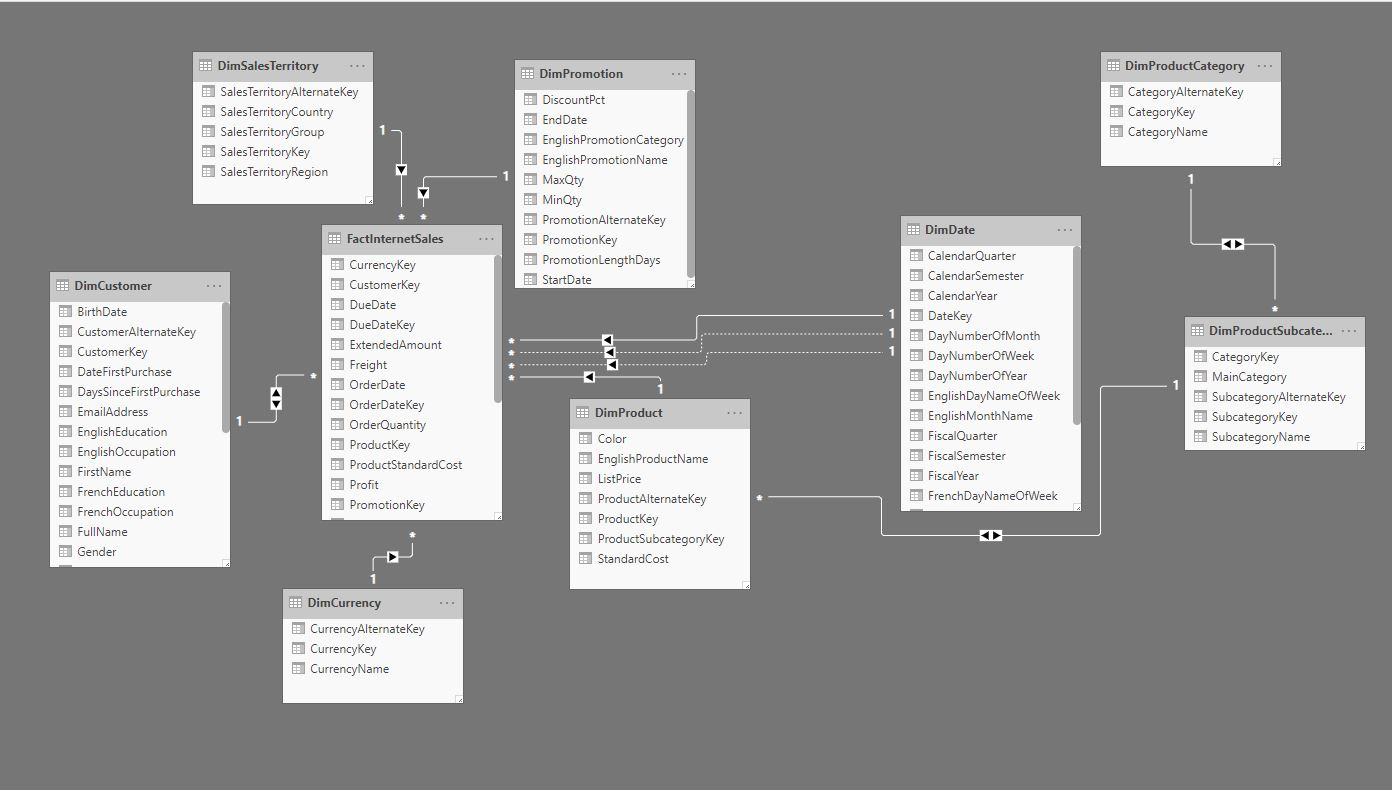
\includegraphics[width=10cm]{./Imagenes/4} 
	\end{center}
\end{itemize} 

\begin{itemize}
	\item Calculo en una columna en la tabla DimProductSubcategory
	\begin{center}
	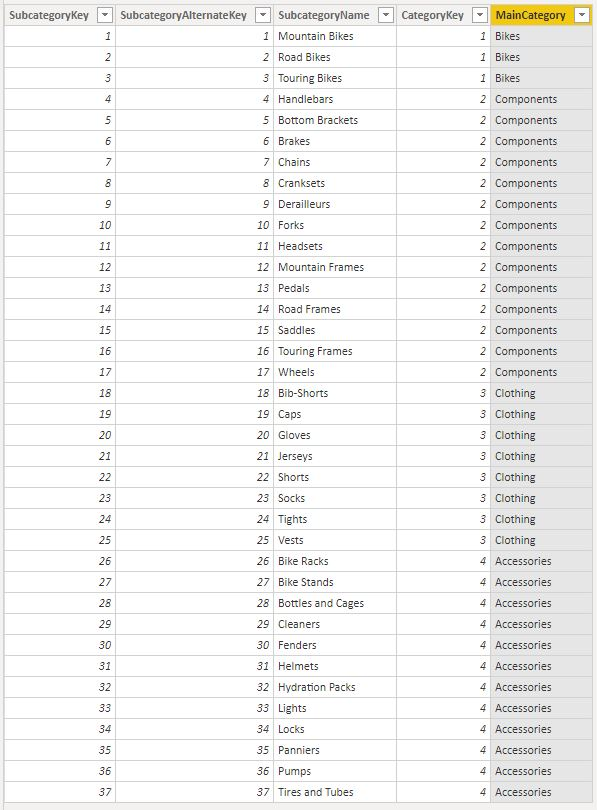
\includegraphics[width=10cm]{./Imagenes/5} 
	\end{center}
\end{itemize} 

\begin{itemize}
	\item Calculo en una columna en la tabla DimPromotion
	\begin{center}
	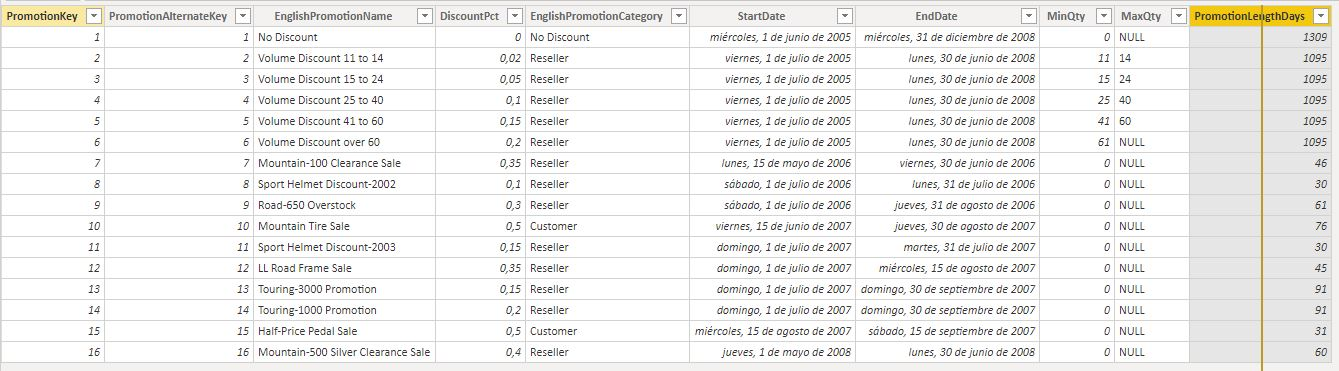
\includegraphics[width=10cm]{./Imagenes/6} 
	\end{center}
\end{itemize} 

\begin{itemize}
	\item Calculo en una columna en la tabla FactInternetSales
	\begin{center}
	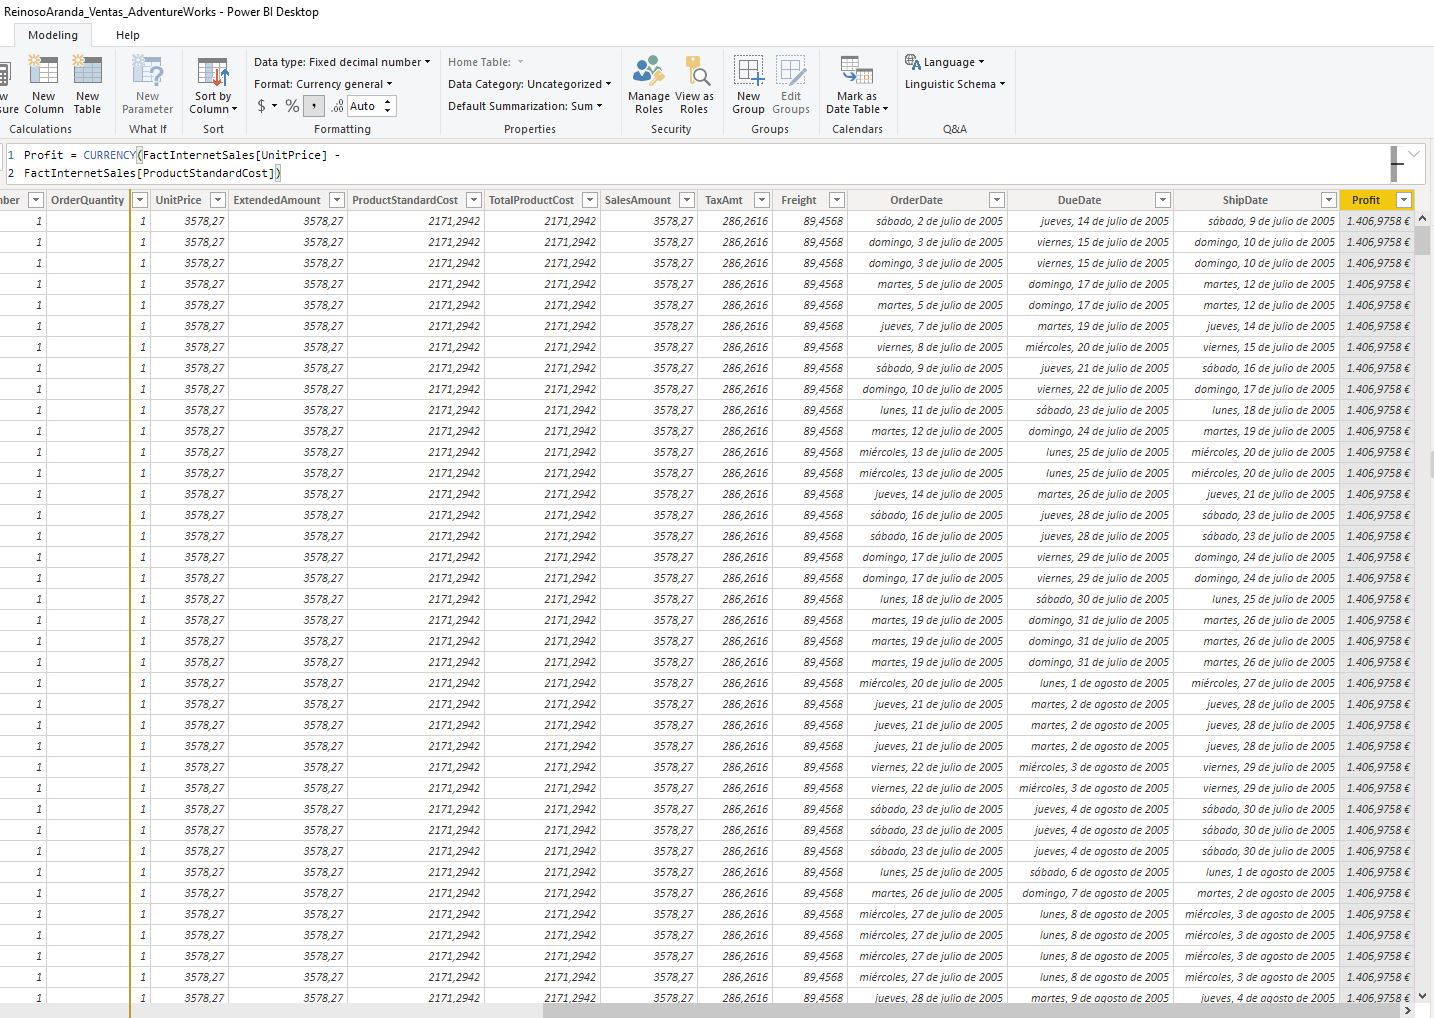
\includegraphics[width=10cm]{./Imagenes/7} 
	\end{center}
\end{itemize} 



\end{document}
